\documentclass{article}

\textwidth=6.5in
\textheight=8.5in
\voffset=-54pt
\oddsidemargin=0in
\evensidemargin=0in
\setlength{\parskip}{8pt}
\setlength{\parindent}{0pt}

\usepackage{workbook}

\usepackage{handout}

\usepackage{exam}

\newcommand{\answerbox}[3][]{
    \fbox{\begin{minipage}[t][#2][c]{#3}
        #1
    \end{minipage}}
    }

\begin{document}

{\large \mbox{} \hfill \bf Name:\underline{\hspace{3in}}}\\[2pt]
{\mbox{} \hfill \it (Please write your name neatly in print.)}\\[12pt]
{\large \mbox{} \hfill \bf HUID:\underline{\hspace{3in}}}
 
\medskip
 
\noindent
{\large\bf
Final Exam Practice 3\\
Math Mb Spring 2025}
\noindent


{\Large
\begin{center}\textbf{Directions---Please read carefully!} \end{center}}

This is a practice test. The same directions will appear on the actual exam, so read them carefully.

\hrulefill 


This exam is subject to the Harvard College Honor Code. No calculators or any other aids are permitted.  Please write as neatly as possible, as answers that can't be read can't be graded and thus can't receive credit. To receive full credit, you must show relevant working
and include units when appropriate. 

You have 180 minutes to complete this exam. 

You may ask for scratch paper if you need additional space to write, but it will not be scanned or graded. Make sure to include all relevant working in this exam booklet in the space provided for each question.

\begin{center}\textbf{Good luck!}\end{center}


\vfill

\centering{
\emph{As a member of Harvard College, I pledge that I will not give or receive assistance on this exam.}}
\vspace{0.3in}

{\large \mbox{} \hfill \bf Signature:\underline{\hspace{3in}}}
\thispagestyle{empty}

\newpage

\begin{enumerate}

\item
  \label{spring2006-midterm2-part2-3-shortened}
  
  Let $h$ be s a differentiable function with a continuous derivative. You are told the following about $h$: 
  \begin{alignat*}{6}
    h'(-4) &= 3 \qquad\qquad & h(-4) &= 1 \qquad\qquad & \int_2^{10}
    h'(x)\,dx &= 7.7 \\
    h'(-1) &= 2 & h(-1) &= -5  \\[8pt]
    h'(1) &= 4 & h(1) &= 3  \\[8pt]
    h' \left( \frac{\pi}{4} \right) & = 7 & h(2) &= 7.5  \\
    & & h(8) &= 0 \vphantom{\int} \\
  \end{alignat*}

  \begin{enumerate}

  \item
    \begin{problem}[\vfill]
      If $\displaystyle f(x) = \sin \left( \frac{\pi}{3} h(x) \right)$,
      find $f'(-1)$. 
    \end{problem}

    \begin{solution}
      We must use the Chain Rule to evaluate $f'(x)$:
      \[ f'(x) = \cos \left( \frac{\pi}{3} h(x) \right) \cdot
      \frac{\pi}{3} h'(x).\]  Plugging in $x = -1$,
      \begin{align*}
        f'(-1) &= \cos \left( \frac{\pi}{3} h(-1) \right) \cdot
        \frac{\pi}{3} h'(-1) \\
        &= \cos \left( -\frac{5 \pi}{3} \right) \cdot \frac{\pi}{3} \cdot
        2 \\
        &= \frac{1}{2} \cdot \frac{\pi}{3} \cdot 2 \\
        &= \boxed{\frac{\pi}{3}}
      \end{align*}
    \end{solution}

  \item
    \begin{problem}[\vfill]
      If $g(x) = h(\tan x)$, find $\displaystyle g' \left( \frac{\pi}{4}
      \right)$. 
    \end{problem}

    \begin{solution}
      We must use the Chain Rule to evaluate $g'(x)$:
      \[ g'(x) = h'(\tan x) \cdot \sec^2 x.\]
      Plugging in $x = \frac{\pi}{4}$,
      \begin{align*}
        g' \left( \frac{\pi}{4} \right) &= h' \left( \tan \frac{\pi}{4}
        \right) \cdot \sec^2 \left( \frac{\pi}{4} \right) \\
        &= h'(1) \cdot 2 \\
        &= \boxed{8}
      \end{align*}
    \end{solution}

  \item
    \begin{problem}[\vfill\newpage]
      Find $\displaystyle \lim_{x \to -4} \frac{\ln [h(x)]}{\arctan (x + 4)}$.
    \end{problem}

    \begin{solution}
      Since $h$ is continuous, as $x \to -4$, $\ln [h(x)] \to \ln [h(-4)]
      = \ln 1 = 0$ and $\arctan(x + 4) \to \arctan 0 = 0$, so we have a
      limit of the indeterminate form $\frac{0}{0}$.  We can use
      L'H\^opital's Rule to help us evaluate this:
      \begin{align*}
        \lim_{x \to -4} \frac{\ln [h(x)]}{\arctan (x + 4)} &
        \stackrel{\text{L'H}}{=} \lim_{x \to -4} \frac{\frac{1}{h(x)}
          \cdot h'(x)}{\frac{1}{1 + (x + 4)^2} \cdot 1}         
      \end{align*}
      Now, as $x \to -4$, the numerator approaches $\frac{h'(-4)}{h(-4)} =
      3$, while the denominator approaches $\frac{1}{1 + 0^2} = 1$, so the
      entire fraction tends to $\boxed{3}$. 
    \end{solution}

  \end{enumerate}

  \continueproblem{\emph{Continued from previous page:}
\begin{alignat*}{6}
    h'(-4) &= 3 \qquad\qquad & h(-4) &= 1 \qquad\qquad & \int_2^{10}
    h'(x)\,dx &= 7.7 \\
    h'(-1) &= 2 & h(-1) &= -5  \\[8pt]
    h'(1) &= 4 & h(1) &= 3  \\[8pt]
    h' \left( \frac{\pi}{4} \right) & = 7 & h(2) &= 7.5  \\
    & & h(8) &= 0 \vphantom{\int} \\
  \end{alignat*}
  }

  \begin{enumerate}[resume]

  \item \label{spring2006-midterm2-part2-3a}
    \begin{problem}[\vfill]
      Find $\displaystyle \int_2^8 h'(x)\,dx$.
    \end{problem}

    \begin{solution}
      By FTOC 2, since $h$ is an antiderivative of $h'$,
      \begin{align*}
        \int_2^8 h'(x)\,dx &= h(x) \Big|_2^8 \\
        &= h(8) - h(2) \\
        &= \boxed{-7.5}
      \end{align*}
    \end{solution}

  \item
    \begin{problem}[\vfill]
      Find $\displaystyle \int_{8}^{10} h'(x)\,dx$.
    \end{problem}

    \begin{solution}
      Since we don't know $h(10)$, we can't use the same strategy as in
      \ref{spring2006-midterm2-part2-3a}.  However, we are given
      $\displaystyle \int_2^{10} h'(x)\,dx$, so let's try to use that:
      \begin{align*}
        \int_8^{10} h'(x)\,dx &= \int_2^{10} h'(x)\,dx - \int_2^8 h'(x)\,dx
        \\
        &= 7.7 - (-7.5) \text{ by \ref{spring2006-midterm2-part2-3a}} \\
        &= \boxed{15.2}
      \end{align*}
    \end{solution}

    \item \label{spring2010-final-9-parts-2} 
    \begin{problem}
      Let $\displaystyle j(x) = \int_2^x h'(t)\,dt$.  Which of the
      following \textbf{must} be true?  Circle all.
      \begin{enumerate}[label=\protect\maybecircle{\Alph*.}]
      \circleitem $j'(x) = h'(x)$
      \plainitem $j(x) = h(x)$
      \circleitem The graphs of $j(x)$ and $h(x)$ are vertical shifts of
        each other.
      \plainitem The graphs of $j(x)$ and $h(x)$ are horizontal shifts of
        each other.
      \end{enumerate}      

      \emph{Note:} If $j(x) = h(x)$, we consider $j(x)$ to be both a
      vertical and a horizontal shift of $h(x)$ (shifted by 0).
    \end{problem}    

    \begin{solution}
      Notice that $j(x)$ is the same as the area function $_2 A_{h'}(x)$,
      so FTOC 1 tells us that $j'(x) = h'(x)$.  From this, it follows that
      the graphs of $j(x)$ and $h(x)$ are vertical shifts of each other.
      (Both $j(x)$ and $h(x)$ are antiderivatives of $h'(x)$, so they must
      differ by a constant.)

      Since $\displaystyle j(2) = \int_2^2 h'(t)\,dt = 0$ while $h(2) =
      7.5$, we see that $j(x)$ \textbf{cannot} equal $h(x)$.
    \end{solution}

  \end{enumerate}  

  \probonly{\newpage}

\item \label{spring2011-final-10-chicken-pox-expanded}

From 1929 to 1970, there were yearly outbreaks of chicken pox in New
  York City.  At the peak of each epidemic (in March of each year), there
  were roughly 1200 cases; at the trough (in September), there were
  roughly 100 cases.  

  \begin{enumerate}
  \item \label{spring2011-final-10-chicken-pox-expanded-model}
    \begin{problem}[\vfill]
      Write a sinusoidal function $C(t)$ that could model the number of
      cases of chicken pox in New York City at time $t$, where $t$ is
      measured in months and $t = 0$ represents September 1929.
    \end{problem}

    \begin{solution}
      From the given information, the graph of $C(t)$ looks like this:
      \begin{center}
        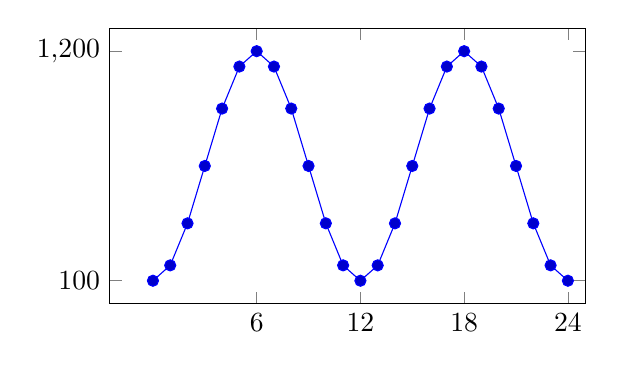
\begin{tikzpicture}
          \begin{axis}[width=3in, height=2in, ytick={100, 1200}, xtick={6,
              12, ..., 24}, xmax=25]
            \addplot+[domain=0:24]{-550*cos(deg(pi*x/6))+650};
          \end{axis}
        \end{tikzpicture}
      \end{center}
      To model this, it's helpful to find the amplitude, midline value,
      and period.  We are told that the period is 12 months.  The
      amplitude is half of the difference between the highest value (1200)
      and lowest value (100), so the amplitude is 550.  The midline value
      is the value half-way between 1200 and 100, which is $650$.

      \begin{checkanswer}
        It's easy to check that our amplitude and midline value are
        consistent: if we add them, we should get the peak population
        (1200), and if we subtract the amplitude from the midline value,
        we should get the lowest population level (100).
      \end{checkanswer}

      Based on our sketch, it makes most sense to model with a vertically
      flipped cosine function, since the function we're modeling has a
      minimum at $t = 0$.  So, the model is $C(t) = -550 \cos \left(
        \frac{2 \pi}{12} t \right) + 650$, which simplifies to $\boxed{-550
        \cos \left( \frac{\pi}{6} t \right) + 650}$.
    \end{solution}

  \end{enumerate}
  Use your sinusoidal model from
  \ref{spring2011-final-10-chicken-pox-expanded-model} to answer the
  following questions. 
  \begin{enumerate}[resume]
  \item
    \begin{problem}[0.75in]
      In June 1930, how many cases of chicken pox were there?
    \end{problem}

    \begin{solution}
      June 1930 is $t = 9$, so we are looking for $C(9) = -550 \cos \left(
        \frac{3 \pi}{2} \right) + 650 = \boxed{650}$.
    \end{solution}

  \item
    \begin{problem}[\vfill\newpage]
      In June 1930, what was the instantaneous rate of change in the
      number of cases of chicken pox?  (Please include units in your
      answer.)
    \end{problem}

    \begin{solution}
      This is asking us for $C'(9)$, which we can compute by first finding
      $C'(t)$: 
      \begin{align*}
        C'(t) &= 550 \sin \left( \frac{\pi}{6} t \right) \cdot
        \frac{\pi}{6} \\
        C'(9) &= 550 \sin \left( \frac{3 \pi}{2} \right) \cdot
        \frac{\pi}{6} \\
        &= \boxed{-550 \cdot \frac{\pi}{6} \text{ cases per month}}
      \end{align*}
    \end{solution}

  \item
    \begin{problem}[\vfill]
      What was the first time after September 1929 at which the number of
      cases reached 375?
    \end{problem}

    \begin{solution}
      We want to solve for the first time at which $C(t) = 375$.
      \begin{align*}
        -550 \cos \left( \frac{\pi}{6} t \right) + 650 &= 375 \\
        -550 \cos \left( \frac{\pi}{6} t \right) &= - 275 \\
        \cos \left( \frac{\pi}{6} t \right) &= \frac{1}{2} \\
        \intertext{To make this look simpler, let's substitute $u =
          \frac{\pi}{6} t$.  We are interested in $t > 0$, which
          corresponds to $u > 0$:}
        \cos u &= \frac{1}{2} \\
        \intertext{The smallest positive value of $u$ that makes this true
          is}
        u &= \frac{\pi}{3} \\
        \intertext{Since $u = \frac{\pi}{6} t$, $t = \frac{6}{\pi} u$}
        t &= \frac{6}{\pi} \cdot \frac{\pi}{3} \\
        &= 2
      \end{align*}
      So, the first time is at $t = 2$, or \fbox{November 1929}. 
    \end{solution}

  \item
    \begin{problem}[\vfill\newpage]
      Find all times between $t = 0$ and $t = 12$ at which the number of
      cases was exactly 870. 
    \end{problem}

    \begin{solution}
      We want to solve $-550 \cos \left( \frac{\pi}{6} t \right) + 650 =
      870$ for $t$ in $[0, 12]$. 
      \begin{align*}
        -550 \cos \left( \frac{\pi}{6} t \right) + 650 &= 870 \\
        -550 \cos \left( \frac{\pi}{6} t \right) &= 220 \\
        \cos \left( \frac{\pi}{6} t \right) &= - \frac{2}{5} \\
        \intertext{To make this look simpler, let's substitute $u =
          \frac{\pi}{6} t$.  We are interested in values of $t$ in $[0,
          12]$, which correspond to values of $u$ in $[0, 2 \pi]$:}% 
        \cos u &= - \frac{2}{5}
      \end{align*}
      We don't know any ``nice'' angles whose cosine is $- \frac{2}{5}$,
      so we'll express our solutions in terms of $\arccos \left( -
        \frac{2}{5} \right)$; let's call this $A$ for short.  Remember
      that $A = \arccos \left( - \frac{2}{5} \right)$ is the angle in $[0,
      \pi]$ whose cosine is $-\frac{2}{5}$; we can picture it like this:
      \begin{center}
        \begin{tikzangle}[angle=rad(acos(-2/5)), label=$\ A$, color=blue,
          func=cos, functick=$-\frac{2}{5}$]
          \draw[blue] (axis cs: 1.5, 0) node[right] {$A = \arccos \left( -
              \frac{2}{5} \right)$}; 
        \end{tikzangle}
      \end{center}
      Then, the solutions of $\cos u = - \frac{2}{5}$ in $[0, 2 \pi]$ are
      these two:
      \begin{center}
        \begin{tabular}{ccc}
          \begin{tikzangle}[angle=rad(acos(-2/5)), func=cos, label=$\ u$,
            functick=$-\frac{2}{5}$] 
          \end{tikzangle}
          &&
          \begin{tikzangle}[angle=rad(acos(-2/5)),
            secondangle=2*pi-rad(acos(-2/5)), func=cos, 
            color=blue, secondcolor=red, seconddistance=0.2, label=$\ A$,
            secondlabel=$u$, functick=$-\frac{2}{5}$, secondlabelpos=0.4]
          \end{tikzangle} \\
          $u = A = \arccos \left( - \frac{2}{5} \right)$ & & $u = 2 \pi -
          A = 2 \pi - \arccos \left( - \frac{2}{5} \right)$
        \end{tabular} 
      \end{center}
      Since $u = \frac{\pi}{6} t$, $t = \frac{6}{\pi} u$, so we get two
      values of $t$, $\boxed{ \frac{6}{\pi}\arccos \left( - \frac{2}{5}
        \right) \text{ and } \frac{6}{\pi} \left[ 2 \pi - \arccos \left(
            - \frac{2}{5} \right) \right]}$. 
    \end{solution}
  \end{enumerate}

\item \label{flu-epidemic}

  
    \newcommand{\graph}{
      \begin{tikzpicture}
        \begin{axis}[gridgraph, xtick={-2, 0, ..., 12}, minor xtick={-1,
            1, ..., 11}, grid=both, minor ytick={-12, -10, ..., 12}, 
          ytick={-12, -8, ..., 12}, width=3.25in, height=2.5in,
          every axis plot/.style={no marks, very thick} ]          
          \addplot+[domain=-2:1] {-6*x-6};
          \addplot+[domain=1:5] {6*(x-1)-12};
          \addplot+[domain=5:7] {12};
          \addplot+[domain=7:12] {-3*(x-11)};
        \end{axis}
      \end{tikzpicture}
    }

    Suppose that there was a flu epidemic in March in Boston, and the
    function $f(t)$ whose graph is shown below represents the \emph{rate of
      change} of the number of flu patients hospitalized at Massachusetts
    General Hospital, in people per day, where $t$ is measured in days and
    $t = 0$ represents noon on March 10.  (So, $t = -1$ is noon on March 9
    and $t = 1$ is noon on March 11.)  At noon on March 12, the hospital had
    60 flu patients.

    \begin{tabular}{c}
      {\small $f(t) = $ rate of change in number of flu patients hospitalized} \\
      {\small (patients per day)} \\
      \graph
    \end{tabular}
    \begin{enumerate}
    \item \label{flu-epidemic-calculate-example} 
      \begin{problem}[\vfill]
        How many flu patients were hospitalized at noon on March 13?
        (Please simplify your answer.)
      \end{problem}

      \begin{solution}
        At noon on March 12 ($t = 2$), the hospital had 60 flu patients.
        Between March 12 and March 13 ($t = 3$) , the net change in the
        number of flu patients was $\displaystyle \int_2^3 f(t)\,dt$.  So,
        the total number of patients hospitalized on March 13 was $60 +
        \displaystyle \int_2^3 f(t)\,dt$.  By interpreting the definite
        integral $\displaystyle \int_2^3 f(t)\,dt$ as a signed area, we see
        that it is equal to $-3$, so $60 + \displaystyle \int_2^3 f(t)\,dt =
        \boxed{57}$.
      \end{solution}

    \item \label{flu-epidemic-increasing} 
      \begin{problem}[\vfill]      
        At what times in $(-2, 12)$ was the number of patients in the
        hospital increasing?
      \end{problem}

      \begin{solution}
        The number of patients is increasing exactly when $f(t)$, the rate
        of change in the number of patients, is positive.  This happens on
        \fbox{$(-2, -1)$ and $(3, 11)$}.
      \end{solution}

    \item
      \begin{problem}[\vfill\newpage]
        At what time in $[-2, 12]$ was the number of hospitalized patients
        the highest?  How many patients were hospitalized at that time? 
      \end{problem}

      \begin{solution}
        In \ref{flu-epidemic-increasing}, we found that the number of
        patients is increasing on $(-2, -1)$ and $(3, 11)$ (and decreasing
        otherwise).  So, the number of patients must be greatest either at
        $t = -1$ or $t = 11$.  The net change in the number of patients
        between $t = -1$ and $t = 11$ is $\displaystyle \int_{-1}^{11}
        f(t)\,dt$, which is positive (we can see this by looking at the graph
        of $f(t)$), which means there are more patients at $\boxed{t =
          11}$.

        We are asked to find the number of patients hospitalized at that
        time, $t = 11$; by the same reasoning as in
        \ref{flu-epidemic-calculate-example}, it is $60 + \displaystyle
        \int_2^{11} f(t)\,dt$.  By interpreting the integral as signed area,
        we find that this is equal to $60 + 57 = \boxed{117}$ patients. 
      \end{solution}

    \end{enumerate}

    \continueproblem{ \emph{Continued from previous page:}

      \begin{tabular}{c}
        {\small $f(t) = $ rate of change in number of flu patients hospitalized} \\
        {\small (patients per day)} \\
        \graph
      \end{tabular}
    }

    \begin{enumerate}[resume]

    \item
      \begin{problem}[1in]
        At what time in $[-2, 12]$ was the number of hospitalized patients
        the lowest?  
      \end{problem}

      \begin{solution}
        In \ref{flu-epidemic-increasing}, we found that the number of
        patients is increasing on $(-2, -1)$ and $(3, 11)$ (and decreasing
        otherwise).  So, the number of patients must be lowest at $t = -2$,
        $t = 3$, or $t = 12$.  From $t = -2$ to $t = 3$, there is a net
        decrease in the number of patients (the signed area under $f$ from
        $-2$ to $3$ is negative), so the number of patients is lower at $t =
        3$ than at $t = -2$.  From $t = 3$ to $t = 12$, there is a net
        increase in the number of patients, so the number of patients is
        lowest at $\boxed{t = 3}$.
      \end{solution}

    \item 
      \begin{problem}
        Let $P(t)$ be the number of patients in the hospital at time $t$.
        Sketch a rough graph of $P(t)$ on $[-2, 12]$.  Please label at least
        one point on the graph with exact coordinates. 

        (\emph{Note:} Your graph need not be completely accurate, but it
        should accurately portray the concavity of $P(t)$ and everything
        else you have found in this problem.)      
      \end{problem}

      \begin{solution}
        We are sketching a function $P(t)$ whose derivative is the given
        function $f(t)$.  We also know that $P(2) = 60$ (at noon on March
        12, the hospital had 60 flu patients). 
        Here is the graph: 
        \begin{center}
          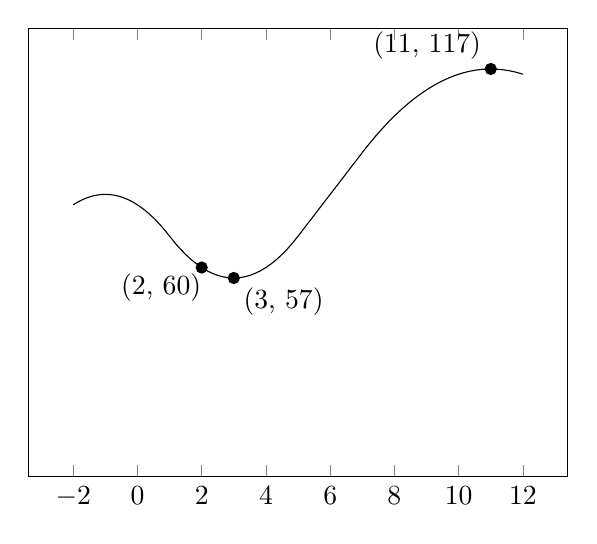
\begin{tikzpicture}
            \begin{axis}[cycle list=black, ymin=0, ytick=\empty]
              \addplot+[domain=-2:1]{-3*x^2-6*x+78};
              \addplot+[domain=1:5]{3*(x-1)^2-12*(x-1)+69};
              \addplot+[domain=5:7]{12*(x-5)+69};
              \addplot+[domain=7:12]{-3/2*(x-11)^2+117};
              \addplot+[only marks] coordinates
              {
                (2, 60) [closed]
                (3, 57) [closed]
                (11, 117) [closed]
              };
              \draw (axis cs: 2, 60) node[anchor=north east, fill=white,
              inner sep=0pt, yshift=-2pt] {(2, 60)};
              \draw (axis cs: 3, 57) node[anchor=north west] {(3, 57)};
              \draw (axis cs: 11, 117) node[anchor=south east] {(11, 117)}; 
            \end{axis}
          \end{tikzpicture}
        \end{center}
        Here are some key features:
        \begin{itemize}
        \item The graph is increasing on $(-2, -1)$ and $(3, 11)$,
          decreasing on $(-1, 3)$ and $(11, 12)$. 
        \item The graph is concave up on $(1, 5)$; concave
          down on $(-2, 1)$ and $(7, 12)$; and linear (of slope $12$) on
          $(5, 7)$.
        \item The absolute minimum point is $(3, 57)$; the absolute maximum
          is $(11, 117)$.
        \end{itemize}
      \end{solution}
\end{enumerate}

\probonly{\newpage}

\item \label{Rachel Epstein problem edited}

The \uline{solar elevation angle} is defined to be the angle between the
  ground and a line from the ground to the sun; it is the angle marked in
  the diagram below.  (Because the sun is so far away from the Earth, it
  doesn't matter exactly where you are on the ground.)  

  \makeatletter

  \pgfdeclareshape{sun}{
    \savedanchor{\centre}{ \pgfpointorigin}
    \anchor{center}{\centre}
    \savedanchor{\top}{
      \pgf@x = 0cm
      \pgf@y = 0.15cm
    }
    \anchor{top}{\top}
    \savedanchor{\bottom}{
      \pgf@x = 0cm
      \pgf@y = -0.375cm
    }
    \anchor{bottom}{\bottom}

    \backgroundpath{
      \foreach \x in {0,45,...,360} {
        \pgfpathmoveto{\pgfpointpolarxy{ \x }{ 1.2 }}
        \pgfpathlineto{ \pgfpointpolarxy{\x }{2 } }
        % \pgfpathcircle{\pgfpointpolarxy{\x}{2.2}}{2pt}
      }   
      \pgfpathcircle{\pgfpointorigin}{1cm}
    }
  }

  \makeatother

  \begin{center}
    \begin{tikzpicture}
      \draw[dashed] (0, 0) -- (4, 2);
      \draw (0, 0) -- node[midway, yshift=-1em]{ground} (4, 0);
      \node [sun, draw, scale=.25, fill=yellow] at (4, 2) {};
      \draw (0.5,0) arc (0:{atan(1/2)}:0.5); 
    \end{tikzpicture}
  \end{center}

  The sun is setting; at precisely 4 pm, the solar elevation angle is
  $\dfrac{\pi}{3}$ radians and shrinking at an instantaneous rate of
  $\dfrac{\pi}{12}$ radians per hour.

  % \begin{enumerate}
  % \item
    \begin{problem}[\newpage]
      There is a $60$-inch-tall woman standing on the ground.  How quickly
      is her shadow changing size at 4 pm?  Is it growing or shrinking?
    \end{problem}

    \begin{solution}
      As usual, let's start by drawing two pictures, a generic
        picture that applies at any time, and a ``snapshot'' showing the
        situation at the time we care about.  We'll also label some
        variables in the generic picture. Let $s$ be the length of the
      shadow and $\theta$ be the solar elevation angle.  
      \begin{center}
        \begin{tabular}{ccc}
          \emph{Generic} & \hspace{0.25in} & \emph{Snapshot} \\
          \begin{tikzpicture}
            \draw[dashed] (0, 0) -- (4, 2);
            \draw (0, 0) -- (4, 0);
            \node [sun, draw, scale=.25, fill=yellow] at (4, 2) {};
            \draw (0.5,0) arc (0:{atan(1/2)}:0.5);
            \draw (3/4, 1/7) node {$\theta$};
            \draw (3, 0) -- node[midway, xshift=3em] { woman (60)} (3,
            1.5);            
            \draw[|-|] (0, -1em) -- node[midway, fill=white]{$s$} (3, -1em);
          \end{tikzpicture} & & 
          \begin{tikzpicture}
            \draw[dashed] (0, 0) -- (4, 2);
            \draw (0, 0) -- (4, 0);
            \node [sun, draw, scale=.25, fill=yellow] at (4, 2) {};
            \draw (0.5,0) arc (0:{atan(1/2)}:0.5);
            \draw (1, 1/5) node {$\pi/3$};
            \draw (3, 0) -- node[midway, xshift=1em] {60} (3, 1.5);
            \draw[|-|] (0, -1em) -- node[midway, fill=white]{$20 \sqrt{3}$} (3, -1em);
          \end{tikzpicture}
        \end{tabular}
      \end{center}
      Note that, in the snapshot, $\displaystyle \tan \frac{\pi}{3} =
      \frac{60}{\text{length of shadow}}$; since we know that $\tan
      \dfrac{\pi}{3} = \sqrt{3}$, we can solve for the length of the shadow
      to get that it is $20 \sqrt{3}$.

      \ideas{Next, we figure out what we know and what we want to know.}

      \highlight{ \textbf{What we know:} $\displaystyle \frac{d\theta}{dt}
        = - \frac{\pi}{12}$ (negative because the angle $\theta$ is
        decreasing)

        \textbf{What we want to know:} $\dfrac{ds}{dt}$
      }

      \ideas{Now, we try to relate variables.  In this case, since the
        rates we know about are $\frac{d\bm{\theta}}{dt}$ and the rate we
        want to know is $\frac{d\bm{s}}{dt}$, we try to relate $\theta$
        and $s$.}

      \highlight{\textbf{Equation relating our variables:} $\displaystyle
        \tan \theta = \frac{60}{s}$ (from our generic picture)}

      \ideas{Once we have our relating equation, we differentiate it.  Since
        we are looking for $\frac{ds}{d\bm{t}}$, we should differentiate
        with respect to $t$.}
      \begin{align*}
        \frac{d}{dt} (\tan \theta) &= \frac{d}{dt} \left( \frac{60}{s}
        \right) \\
        \frac{d}{dt} (\tan \theta) &= \frac{d}{dt} \left( 60 s^{-1}
        \right) \\
        \sec^2 \theta \frac{d\theta}{dt} &= - 60 s^{-2} \frac{ds}{dt}
        \intertext{Now, we can plug in the snapshot information.}
        \sec^2 \left( \frac{\pi}{3} \right) \cdot \left( - \frac{\pi}{12}
        \right) &= - \frac{60}{(20 \sqrt{3})^2} \frac{ds}{dt} \\
        \intertext{We know that $\sec \frac{\pi}{3} = \frac{1}{\cos
            \frac{\pi}{3}} = \frac{1}{1 / 2} = 2$:}
        2^2 \left( - \frac{\pi}{12} \right) &= - \frac{1}{20} \frac{ds}{dt}
        \\
        \frac{20 \pi}{3} &= \frac{ds}{dt}
      \end{align*}
      So, the shadow length is \fbox{increasing at a rate of $\dfrac{20
          \pi}{3}$ inches per hour} (we know that the shadow length is
      increasing because we calculated that $\frac{ds}{dt}$ is positive).
    \end{solution}

  % \item 
  %   \begin{problem}[\newpage]
  %     At the same time, you notice a man sinking in the mud at a rate of 2
  %     inches per hour.  At 4 pm, only his feet have been submerged, and he
  %     still stands 70 inches above the ground.  Considering the rate at
  %     which he is shrinking and the rate at which the sun is setting, at
  %     what rate is the length of his shadow changing?

  %     (\emph{Note:} Since we are still considering the situation at 4 pm,
  %     it's still true that the solar elevation angle is $\dfrac{\pi}{3}$
  %     and shrinking at an instantaneous rate of $\dfrac{\pi}{12}$ radians
  %     per hour.)
  %   \end{problem}

  %   \begin{solution}
  %     \ideas{Again, let's draw a generic picture and a ``snapshot''
  %       picture.}  Let $s$ be the length of the shadow, $h$ be the man's height above
  %   the ground (which is changing in this scenario), and $\theta$ be the
  %   solar elevation angle.
  %   \begin{center}
  %     \begin{tabular}{ccc}
  %       \emph{Generic} & \hspace{0.25in} & \emph{Snapshot} \\
  %       \begin{tikzpicture}
  %         \draw[dashed] (0, 0) -- (4, 2);
  %         \draw (0, 0) -- (4, 0);
  %         \node [sun, draw, scale=.25, fill=yellow] at (4, 2) {};
  %         \draw (0.5,0) arc (0:{atan(1/2)}:0.5);
  %         \draw (3/4, 1/7) node {$\theta$};
  %         \draw (3, 0) -- node[midway, xshift=0.5em] {$h$} (3,
  %         1.5);            
  %         \draw[|-|] (0, -1em) -- node[midway, fill=white]{$s$} (3, -1em);
  %       \end{tikzpicture} & & 
  %       \begin{tikzpicture}
  %         \draw[dashed] (0, 0) -- (4, 2);
  %         \draw (0, 0) -- (4, 0);
  %         \node [sun, draw, scale=.25, fill=yellow] at (4, 2) {};
  %         \draw (0.5,0) arc (0:{atan(1/2)}:0.5);
  %         \draw (1, 1/5) node {$\pi/3$};
  %         \draw (3, 0) -- node[midway, xshift=1em] {70} (3, 1.5);
  %         \draw[|-|] (0, -1em) -- node[midway, fill=white]{$70 / \sqrt{3}$} (3, -1em);
  %       \end{tikzpicture}
  %     \end{tabular}
  %   \end{center}

  %   \ideas{Next, we figure out what we know and what we want to know.}

  %   \highlight{ \textbf{What we know:} $\displaystyle \frac{d\theta}{dt}
  %     = - \frac{\pi}{12}$ (negative because the angle $\theta$ is
  %     decreasing), $\displaystyle \frac{dh}{dt} = -2$ (negative because
  %     the man's height above the ground is decreasing) 

  %     \textbf{What we want to know:} $\dfrac{ds}{dt}$
  %   }

  %   \ideas{Now, we try to relate variables.  In this case, since the
  %     rates we know about are $\frac{d\bm{\theta}}{dt}$ and
  %     $\frac{d\bm{h}}{dt}$ and the rate we want to know is
  %     $\frac{d\bm{s}}{dt}$, we try to relate $\theta$, $h$, and $s$.}

  %   \highlight{\textbf{Equation relating our variables:} $\displaystyle
  %     \tan \theta = \frac{h}{s}$ (from our generic picture)}

  %   \ideas{Once we have our relating equation, we differentiate it.  Since
  %     we are looking for $\frac{ds}{d\bm{t}}$, we should differentiate
  %     with respect to $t$.}
  %   The equation will be slightly easier to differentiate if we first
  %   multiply both sides by $s$ (then we won't need the Quotient Rule):
  %   \begin{align*}
  %     s \tan \theta &= h \\
  %     \frac{d}{dt} (s \tan \theta) &= \frac{d}{dt} (h) \\
  %     s \sec^2 \theta \frac{d\theta}{dt} + \frac{ds}{dt} \tan \theta &=
  %     \frac{dh}{dt} \\
  %     \intertext{Now, we can plug in the snapshot information.}  %
  %     \frac{70}{\sqrt{3}} \sec^2 \left( \frac{\pi}{3} \right) \cdot \left
  %       (- \frac{\pi}{12} \right) + \frac{ds}{dt} \tan \left(
  %       \frac{\pi}{3} \right) &= -2
  %     \\
  %     \frac{70}{\sqrt{3}} \cdot 4 \cdot \left (- \frac{\pi}{12} \right) +
  %     \sqrt{3} \frac{ds}{dt} &= -2
  %     \\
  %     \sqrt{3} \frac{ds}{dt} &= \frac{70 \pi}{3 \sqrt{3}} - 2 \\
  %     \frac{ds}{dt} &= \frac{70 \pi}{9} - \frac{2}{\sqrt{3}}
  %   \end{align*}
  %   This is positive, so the length of the man's shadow is
  %   \fbox{increasing at a rate of $\displaystyle \frac{70 \pi}{9} -
  %     \frac{2}{\sqrt{3}}$ inches/hr}.
  %   \end{solution}

  % \end{enumerate}

  \item \label{2018practice2}
 
 Pebble Pond, a round pond with radius 3 kilometers (km), sits at the center of a small town. The population density of the town varies with $x$, the distance in kilometers from the \textit{edge} of the pond, and is given by $\rho(x)$ people per square kilometer. We are interested in figuring out how many people live within 50 km of the center of the pond. Note carefully that nobody lives {\it in} the pond, and the farthest away anyone lives from the \textit{edge} of the pond is 47 km. 

\begin{enumerate}
\item Write a general Riemann Sum that estimates the number of people living within 50 kilometers of the center of Pebble Pond. Draw a clear and labeled picture to show how you are slicing. If you use expressions like $n$, $\Delta x$, $x_k$, $\Delta r$, or $r_k$, let us know how you defined them. 


\begin{solution}

\begin{center}
\[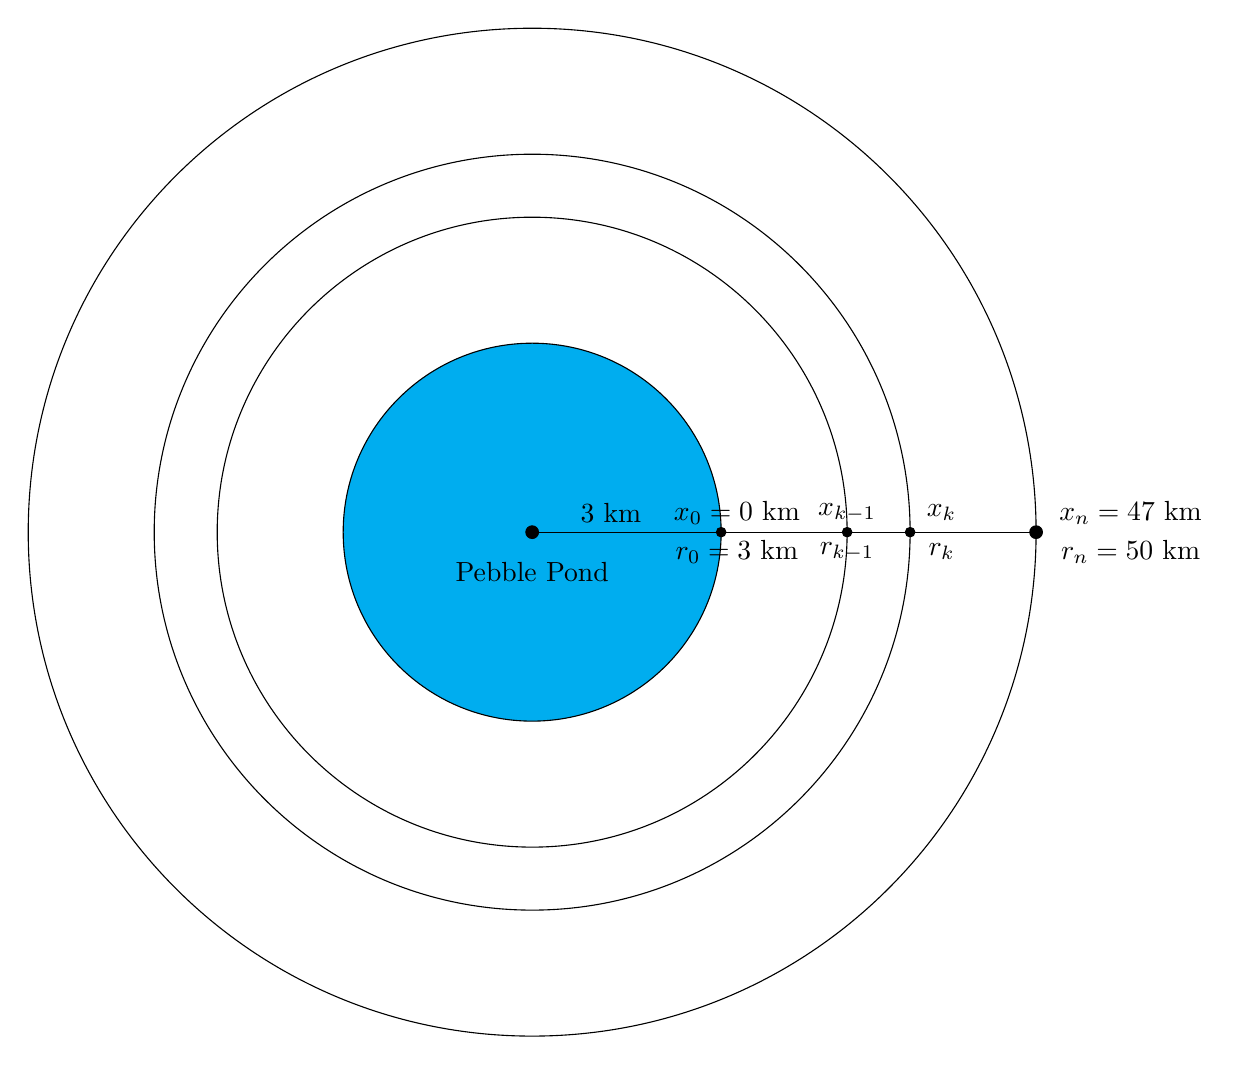
\begin{tikzpicture}
\draw [fill=cyan] (0,0) circle (2.4cm);
\draw (0,0) circle (4cm);

\draw (0,0) circle (4.8cm);
\draw (0,0) circle (6.4cm);
\draw (0,0) -- (6.4,0);

\draw [fill] (0,0) circle [radius=.08];
\node at (0,-.5){Pebble Pond};
\node at (1,0.25) {3 km};
\draw [fill] (2.4,0)circle [radius=.06];
\node at (2.6,.25){$x_0=0$ km};
\node at (2.6,-.25){$r_0=3$ km};
\draw [fill] (4,0)circle [radius=.06];
\node at (4,.25){$x_{k-1}$};
\node at (4,-.25){$r_{k-1}$};
\draw [fill] (4.8,0)circle [radius=.06];
\node at (5.2,.25){$x_k$};
\node at (5.2,-.25){$r_k$};
\draw [fill] (6.4,0) circle [radius=.08];
\node at (7.6,0.25){$x_n = 47$ km};
\node at (7.6,-0.25){$r_n = 50$ km};
\end{tikzpicture}\]
\end{center}

We slice the town around the pond into concentric rings, so the density of people within each slice is roughly constant. For the $k$th slice, let $x_k$ be the distance between the slice and the edge of the pond, and let $r_k$ be the radius of the slice, which is the distance from the center of the pond to the $k$th slice. Then $a=x_0=0$ km and $b=x_n=47$ km. Thus,
$\Delta x = \frac{47}{n}$ and $x_k=k\Delta x$.

The circumference of the $k$th slice is $2 \pi r_k$, where $r_k=x_k+3$, since $r_k$ must also include the radius of Pebble Pond at the center of the town. Thus, the area of the $k$th slice is approximated by $2 \pi r_k \Delta x = 2\pi (x_k+3)\Delta x$. The density of the $k$th slice is $\rho(x_k)$. Hence the approximate population on the $k$th slice is

\[ 2 \pi (x_k+3)  \rho(x_k) \Delta x \]

So the Riemann sum approximating the total population is

\[ \boxed{\sum_{k=1}^n 2 \pi (x_k+3)  \rho(x_k) \Delta x} \]

You could have also written the Riemann sum in terms of $r$ as follows:

$$\boxed{\sum_{k=1}^n 2 \pi (r_k)  \rho(r_k-3) \Delta r} $$

Here are some things you always want to see in a Riemann sum: first, you must see a $\Delta x$ term, but never a $\Delta x^2$ or anything like that. Secondly, you must have only $x_k$ and $\Delta x$ terms, never $x$ by itself. Finally, you want everything converted into one variable. You may use $r_k,\Delta r$ or $x_k, \Delta x$ but no mixing of these.
\end{solution}

\probonly{\vfill}

\item 
\begin{problem}[1in]
    Explicitly take the limit of the general Riemann sum from part (a) to arrive at an integral giving the number of people living within 50 kilometers of the center of Pebble Pond.
\end{problem} 

\begin{solution}
When turning a Riemann sum into an integral, you must remember the bounds of the integration. This is not contained in the Riemann sum notation. In this question, $x$ ranges from $0$ to $47$ while $r$ ranges from $3$ to $50$. Note the Riemann sums have no mention of $0$, $3$, $47$, or $50$, so you have to remember this from the values $x_0$, $x_n$, $r_0$, and $r_n$. 

By taking the limit as $n \to \infty$ of the above Riemann sums, we get the following integrals:

\[\lim_{n \to \infty}\sum_{k=1}^n 2 \pi (x_k+3)  \rho(x_k) \Delta x = \boxed{\int_0^{47} 2 \pi (x+3)  \rho(x) dx} \]
or 
\[\lim_{n \to \infty}\sum_{k=1}^n 2 \pi (r_k)  \rho(r_k-3) \Delta r = \boxed{\int_3^{50} 2 \pi r \rho(r - 3) dr}\]
\end{solution}

\end{enumerate}

\probonly{\newpage}

\item
  \label{spring2012-mb-midterm2-proposed-implicit-differentiation-trig}

The picture below shows a portion of the curve given by the equation
  \[ (\arctan x)(\sin y)=\frac{\pi}{8}.\] A point $P$ on the curve is
  marked.
  \begin{center}
    
\includegraphics[height=2in]{assessments/Final Exam/Practice Exams/spring2012-mb-midterm2-proposed-implicit-differentiation-trig.png}
  \end{center}

  \begin{enumerate}
  \item
    \begin{problem}[1.25in]
      The point $P$ has $x$-coordinate $1$.  Find the $y$-coordinate of
      $P$.
    \end{problem}

    \begin{solution}
      The point $P$ is a point on the curve
      \begin{align*}
        (\arctan x) (\sin y) &= \frac{\pi}{8} \\
        \intertext{We know that its $x$-coordinate is 1:}
        (\arctan 1) (\sin y) &= \frac{\pi}{8} \\
        \frac{\pi}{4} \cdot \sin y &= \frac{\pi}{8} \\
        \sin y &= \frac{1}{2} \\
        \intertext{There are infinitely many values of $y$ satisfying
          $\sin y = \frac{1}{2}$, but we can see from the graph that the
          one we want is 
          between $-3$ and $-4$:} %
        y &= \boxed{- \frac{7 \pi}{6}}
      \end{align*}
    \end{solution}

  \item
    \begin{problem}[\vfill\newpage]
      Find an equation for the line tangent to the curve at the point
      $P$. 
    \end{problem}

    \begin{solution}
      The slope of the line we're looking for is $\frac{dy}{dx}$ at
      $\left( 1, - \frac{7 \pi}{6} \right)$.  We can use implicit
      differentiation to find this:
      \begin{align*}
        (\arctan x) (\sin y) &= \frac{\pi}{8} \\
        \intertext{Differentiate both sides with respect to $x$:}
        \frac{d}{dx} \left(\fcolorbox{green}{white}{$\displaystyle
            \arctan(x)$}\cdot
          \fcolorbox{green}{white}{$\displaystyle  \sin
            \left(y\right)$}\right) &= \frac{d}{dx} \left( \frac{\pi}{8}
        \right) \\
        \arctan(x)\cdot \frac{d}{dx}
        \left(\fcolorbox{red}{white}{$\displaystyle \sin
            \left(\fcolorbox{blue}{white}{$\displaystyle
                y$}\right)$}\right)+ \frac{1}{x^2+1}\cdot \sin
        \left(y\right) &= 0 \\ 
        \arctan(x)\cdot \left(\cos \left(y\right)\cdot 
          \frac{dy}{dx}\right)+ \frac{1}{x^2+1}\cdot \sin \left(y\right)
        &= 0 \\
        \shortintertext{Now, we plug in the point we care about:}
        \arctan (1) \cdot \cos \left( - \frac{7 \pi}{6} \right) \cdot
        \frac{dy}{dx} + \frac{1}{2} \cdot \sin \left( - \frac{7 \pi}{6}
        \right) &= 0 \\
        \frac{\pi}{4} \left( - \frac{\sqrt{3}}{2} \right) \frac{dy}{dx} +
        \frac{1}{2} \cdot \frac{1}{2} &= 0 \\
        - \frac{\pi \sqrt{3}}{8} \frac{dy}{dx} &= - \frac{1}{4} \\
        \frac{dy}{dx} &= \frac{2}{\pi \sqrt{3}}
      \end{align*}
      This is the slope of the tangent line; we also know that the line
      goes through the point $\left( 1, - \frac{7 \pi}{6} \right)$, so the
      equation of the line we want is $\boxed{y + \frac{7 \pi}{6} =
        \frac{2}{\pi \sqrt{3}} \left(x - 1 \right)}$.

      \begin{checkanswer}
        From the picture, we can see that the slope of this tangent line
        should be positive.
      \end{checkanswer}
    \end{solution}

  \end{enumerate}

  \item \label{2018practice4}
  
  Find the dimensions of the largest rectangle (i.e., the rectangle with the most area) that can be inscribed in a semicircle with radius 100. Justify your answer. (\textit{Hint: Draw in a useful right triangle!})

\begin{multicols}{2}
     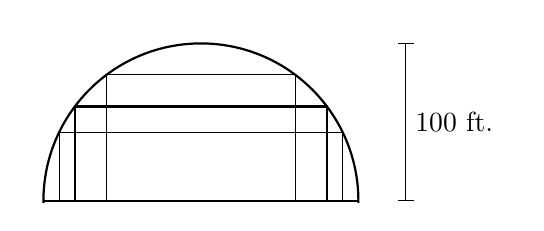
\begin{tikzpicture}[scale=2]
        \clip (-1.1,-.01) rectangle (2,1.1);
        \draw[thick] (0,0) circle(1);
        \draw[thick] (-1,0) -- (1,0);
        \draw[thick] (-.8,0) rectangle (.8,.6);
        \draw (1.3,0) -- (1.3, 1);
        \draw (1.25,0) -- (1.35,0);
        \draw (1.25,1) -- (1.35,1);
        \node[right] at (1.3,0.5) {100 ft.};
        \draw[thin] (-.9,0) rectangle (.9,.436);
        \draw[thin] (-.6,0) rectangle (.6,.8);
    \end{tikzpicture}
    
    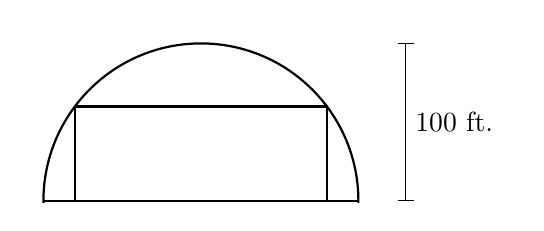
\begin{tikzpicture}[scale=2]
        \clip (-1.1,-.01) rectangle (2,1.1);
        \draw[thick] (0,0) circle(1);
        \draw[thick] (-1,0) -- (1,0);
        \draw[thick] (-.8,0) rectangle (.8,.6);
        \draw (1.3,0) -- (1.3, 1);
        \draw (1.25,0) -- (1.35,0);
        \draw (1.25,1) -- (1.35,1);
        \node[right] at (1.3,0.5) {100 ft.};
        %\draw[thick, domain=-1:1, samples=100] plot (\x, sqrt(1-\x*\x));
        %\draw[thick, domain=-1:1] plot (\x, 0);
    \end{tikzpicture}
\end{multicols}
        
\begin{solution}

\textbf{Goal:} Maximize the area of the rectangle.

\textbf{Function to optimize:} If we label $x$ and $y$ as shown in the picture below, the area of the rectangle is given by $\displaystyle A=2xy$.  However, in order to optimize $A$ we need to express it in terms of one variable.  Thus we will need a relationship between $x$ and $y$.


        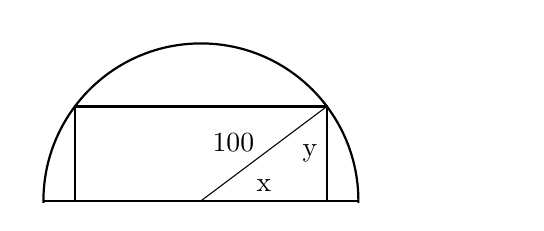
\begin{tikzpicture}[scale=2]
        \clip (-1.1,-.01) rectangle (2,1.1);
        \draw[thick] (0,0) circle(1);
        \draw[thick] (-1,0) -- (1,0);
        \draw[thick] (-.8,0) rectangle (.8,.6);
        \draw (0,0) -- (.8,.6);
        \node[above] at (.4,0) {x};
        \node[left] at (.8,.3) {y};
        \node[above left] at (.4,.25) {100};
    \end{tikzpicture}
    
\textbf{Constraint equation:} Since 100 is the radius of the semicircle, it is the hypotenuse of the triangle with legs $x$ and $y$.  This gives the constraint $\displaystyle x^2+y^2=100^2$, or $y=\sqrt{100^2-x^2}$.

\textbf{Function to optimize (in one variable):}
\begin{align*}
    A=2x\sqrt{100^2-x^2}
\end{align*}

\textbf{Maximize} To find the critical points, we first set $A'=0$:
\begin{align*}
    \frac{dA}{dx}=2\left(x\cdot\frac{1}{2}(100^2-x^2)^{-1/2}\cdot -2x + 1\cdot\sqrt{100^2-x^2}\right) &= 0 \\
    2\left(\frac{-x^2}{\sqrt{100^2-x^2}} + \sqrt{100^2-x^2}\right) &= 0 \\
    \sqrt{100^2-x^2} &= \frac{x^2}{\sqrt{100^2-x^2}} \\
    100^2 - x^2 &= x^2 \\
    100^2 &= 2x^2 \\
    x^2 &= 5000 \\
    x &= \sqrt{5000}
\end{align*}

First, we determine whether this is truly a maximum.  The domain of $x$ is $[0,100]$, so the endpoints 0 and 100 are critical points. $A'$ is defined on the open interval $(0,100)$, so $\sqrt{5000}$ is the only critical point between the endpoints.  If we plug in 1 we get $A'>0$ and if we plug in 99 we get $A'<0$, which tells us $\sqrt{5000}$ is indeed an absolute maximum.
    
Now solve for $y$ using the constraint equation:
\begin{align*}
    (\sqrt{5000})^2 + y^2 &= 100^2 \\
    5000 + y^2 &= 10000 \\
    y^2 &= 5000 \\
    y &= \sqrt{5000}
\end{align*}

Thus the dimensions of the rectangle with maximal area are $2\sqrt{5000} \textrm{ ft.} \times \sqrt{5000} \textrm{ ft.}$
\end{solution}  

\probonly{\newpage}

\item \label{diffeq-interest-modeling-abc EDITED} 

Bernardo and Clementina each have \$1000 to invest, but they
  decide on very different investment strategies.

  \begin{enumerate}
  
  \item
    \begin{problem}[1in]
      Bernardo puts his money in an account that guarantees a nominal
      annual interest rate of 2\%, compounded \emph{continuously}.  If $B(t)$ is the amount of money in Bernardo's account at time $t$, where $t$ is given in years, write a differential equation that models the situation.
    \end{problem}

    \begin{solution}
Saying that an account earns a
      nominal annual interest rate of 2\%, compounded continuously,
      exactly means that
      \[ \text{rate at which account earns money} = (2\%) (\text{amount of
        money})\]
      If we let $B(t)$ be the amount of money Bernardo has at time $t$, we
      can write this as
      \[ \frac{dB}{dt} = 0.02 B\]
    \end{solution}

    \item 
    \begin{problem}[\vfill] Write a formula for $B(t)$.
    \end{problem}
    \begin{solution}
    You should recognize the solution of this differential equation as
      having the form $B(t) = C e^{0.02 t}$.  Since we are told that
      Bernardo has an initial balance of \$1000, we know that $B(t) =
      \boxed{ 1000 e^{0.02 t}}$. 
    \end{solution}

  \item 
  \begin{problem}[2in]
      Clementina puts her money in an account with a nominal annual
    interest rate of 2\%, compounded continuously, but she plans to
    withdraw \$10 a month. The differential equation that models $C(t)$, the amount of
        money in Clementina's account after $t$ years, is: $\frac{dC}{dt} = 0.02 C - 120$
        
        Which of the following gives the amount of money Clementina has in
        her account after $t$ years?
        \begin{enumerate}[label=\protect\maybecircle{\Alph*.}]
        \plainitem $(1000 + 10t) e^{0.02 t}$
        \plainitem $1000 e^{0.02 t} + 120 t$
        \circleitem $6000 - 5000 e^{0.02 t}$
        \plainitem $6000 + 5000 e^{-0.02 t}$
        \end{enumerate}          
      \end{problem}

      \begin{solution}
        We are looking for the choice that satisfies our differential
        equation $\frac{dC}{dt} = 0.02 C - 120$ \emph{and} initial
        condition $C(0) = 1000$.   
        \begin{enumerate}
            \plainitem If $C(t)=(1000 + 10t) e^{0.02 t}$, then $C(0)=(1000+0)\cdot 1=1000$, so choice (A) satisfied our initial condition. Let's check if it also satisfies our differential equation $\frac{dC}{dt} = 0.02 C - 120$: 
            \begin{align*}
          \frac{d}{dt} \left( (1000 + 10t) e^{0.02 t} \right) &
          \stackrel{?}{=} 0.02 \left( (1000 + 10t) e^{0.02 t} \right) -
          120 \\
          (1000+10t) \left(0.02 e^{0.02 t} \right) + 10 e^{0.02t}& \stackrel{?}{=} (1000+10t) \left(0.02 e^{0.02 t} \right) - 120
        \end{align*}
        We can see that $\frac{dC}{dt} \neq 0.02 C - 120$ so choice (A) is not the right function.
            
            \plainitem If $C(t)=1000 e^{0.02 t} + 120 t$ then $C(0)=(1000\cdot 1)+0=1000$, so choice (B) satisfies our initial condition. Let's check if it also satisfies our differential equation: 

            \begin{align}
                \frac{d}{dt} \left( 1000 e^{0.02 t} + 120 t \right) &
          \stackrel{?}{=} 0.02 \left( 1000 e^{0.02 t} + 120 t \right) -
          120 \\
          20 e^{0.02 t} + 120 &
          \stackrel{?}{=} 20e^{0.02 t} + 2.4 t -
          120
            \end{align}

            Again, $\frac{dC}{dt} \neq 0.02 C - 120$ so choice (B) is not a solution.
            
            \plainitem $6000 - 5000 e^{0.02 t}$
            If $C(t) = 6000 - 5000 e^{0.02 t}$, then $C(0) =
        6000 - 5000 = 1000$, so choice (C) at least satisfies our initial
        condition.  Let's check that it also satisfies our differential
        equation $\frac{dC}{dt} = 0.02 C - 120$:
        \begin{align*}
          \frac{d}{dt} \left( 6000 - 5000 e^{0.02 t } \right) &
          \stackrel{?}{=} 0.02 \left( 6000 - 5000 e^{0.02 t } \right) -
          120 \\
          - 5000 \left(0.02 e^{0.02 t} \right) & \stackrel{?}{=} 120 -
          0.02 \cdot 5000 e^{0.02 t} - 120
        \end{align*}
        This equation is true, so $C(t) = 6000 - 5000 e^{0.02 t}$ is a solution to our differential equation!
            
            \plainitem If $C(t)=6000 + 5000 e^{-0.02 t}$, then $C(0)=6000+5000=11000$, so choice (D) does not satisfy our initial condition.
        \end{enumerate}

      \end{solution}

    \end{enumerate}

\probonly{\newpage}

\item \label{spring2011-final-revisit-qualifying-7}

\begin{enumerate}

\item \label{spring2011-final-revisit-qualifying-7-sketch}
    \begin{problem}[\vfill]
      Sketch $y = \arcsin x$. Make your sketch very large, and make sure the
      domain, range, and intercepts of your graph are clear.
    \end{problem}

    \begin{solution}
      Remember that we get $\arcsin x$ by taking the graph of $\sin x$
      (shown in black below), restricting it to the domain $\left[ -
        \frac{\pi}{2}, \frac{\pi}{2} \right]$ (shown in red), and then
      flipping it over the line $y = x$ (which flips the $x$- and
      $y$-coordinates of each point).  So, the graph of $\arcsin x$ is the
      blue graph below:
      \begin{center}
        \begin{tikzpicture}
          \begin{axis}[xtick={-4.71239, -3.14159, -1.5708, 0., 1.5708,
              3.14159, 4.71239}, xticklabels={$-\frac{3 \pi }{2}$, $-\pi$,
              $-\frac{\pi }{2}$, $0.$, $\frac{\pi }{2}$, $\pi$, $\frac{3
                \pi }{2}$}, ytick={-4.71239, -3.14159, -1.5708, 0.,
              1.5708, 3.14159, 4.71239}, yticklabels={$-\frac{3 \pi }{2}$,
              $-\pi$, $-\frac{\pi }{2}$, $0.$, $\frac{\pi }{2}$, $\pi$,
              $\frac{3 \pi }{2}$}, clip=false, axis equal=true, width=3.75in,
            height=2.25in]
            \addplot[gray, dashed, domain=-2.25:2.25] {x} node[right]{$y = x$};
            \addplot+[domain=-5:5] {sin(deg(x))};
            \addplot+[domain=-pi/2:pi/2, red, very thick]{sin(deg(x))};
            \addplot+[domain=-1:1, blue, very thick]{rad(asin(x))};
            \addplot[closed, red] coordinates
            {
              ({pi/2}, 1)
              ({-pi/2}, -1)
            }
            node[pos=0, anchor=south west]{$\left( \frac{\pi}{2}, 1 \right)$}
            node[pos=1, anchor=north east]{$\left(- \frac{\pi}{2}, -1 \right)$};            
            \addplot[only marks, mark=*, blue, mark size=1.5pt] coordinates
            {
              (-1, {-pi/2})
              (1, {pi/2})
            }
            node[pos=0, below]{$\left(1, \frac{\pi}{2} \right)$}
            node[pos=1, above]{$\left(-1, - \frac{\pi}{2} \right)$};            
          \end{axis}
        \end{tikzpicture}
      \end{center}
      In particular, the domain is $[-1, 1]$, and the range is $\left[ -
        \frac{\pi}{2}, \frac{\pi}{2} \right]$. 
    \end{solution}

  \item \label{spring2011-final-revisit-qualifying-7-sketch-integral}
    \begin{problem}[\vfill]
      On the graph you sketched in
      \ref{spring2011-final-revisit-qualifying-7-sketch}, the graph of $y
      = \arcsin x$, lightly shade the region corresponding to
      $\displaystyle \int_{0.2}^{0.6} \arcsin x\,dx$.
    \end{problem}

    \begin{solution}
      \begin{center}
        \begin{tikzpicture}
          \begin{axis}[x=1.5cm, y=1.5cm, ytick={-1.57, 1.57},
            yticklabels={$-\frac{\pi}{2}$, $\frac{\pi}{2}$}, xtick={-1,
              0.2, 0.6, 1}, enlarge x limits=0.04]
            \addplot+[domain=0.2:0.6, plusarea] {rad(asin(x))} \closedcycle;
            \addplot+[domain=-1:1] {rad(asin(x))};
          \end{axis}
        \end{tikzpicture}
      \end{center}
    \end{solution}

  \item \label{spring2011-final-revisit-qualifying-7-sketch-L4} 
    \begin{problem}[\vfill\newpage]
      Draw a pictorial representation of $L_4$, the left hand sum with 4
      terms that approximates the integral $\displaystyle \int_{0.2}^{0.6}
      \arcsin x\,dx$.
    \end{problem}

    \begin{solution}
      $L_4$ is the area in the rectangles:
      \begin{center}
        \begin{tikzpicture}[declare function={f(\x)=rad(asin(\x));}]
          \begin{axis}[x=1.5cm, y=1.5cm, ytick={-1.57, 1.57},
            yticklabels={$-\frac{\pi}{2}$, $\frac{\pi}{2}$}, xtick={-1,
              0.2, 0.6, 1}, enlarge x limits=0.04]
            \addplot+[domain=-1:1] {f(x)};
            \addplot+[ybar interval, plusarea] coordinates { (0.2,
              {f(0.2)}) (0.3, {f(0.3)}) (0.4, {f(0.4)}) (0.5, {f(0.5)})
              (0.6, {f(0.5)}) }; 
          \end{axis}
        \end{tikzpicture}
      \end{center}
    \end{solution}

  \item
    \begin{problem}[\newpage]
      Put the following in order from smallest to largest, using ``$<$''
      or ``$=$'' signs between them.  (You may use the letters, like ``$A
      < B = C \ldots$''.)
      \begin{enumerate}[label=\Alph*.]
      \item $\displaystyle \int_{0.2}^{0.6} \arcsin x\,dx$
      \item $\displaystyle \int_{0}^{1} \arcsin x\,dx$    
      \item $\displaystyle \int_{0}^{-0.3} \arcsin x\,dx$ 
      \item $\displaystyle \int_{-1}^1 \arcsin x\,dx$
      \item $\displaystyle \int_{-1}^0  \arcsin x\,dx$
      \item $\displaystyle \int_{-0.3}^0\arcsin x\,dx$
      \item $\displaystyle \arcsin (0.2) 0.1 + \arcsin (0.3) 0.1
        +\arcsin (0.4) 0.1 +\arcsin (0.5) 0.1$
      \item $\displaystyle \arcsin (0.3) 0.1 +\arcsin (0.4) 0.1 +\arcsin
        (0.5) 0.1+ \arcsin (0.6) 0.1$
      \end{enumerate}      
    \end{problem}

    \begin{solution}
      Let's think about these individually.
      \begin{enumerate}[label=\Alph*.]
      \item $\displaystyle \int_{0.2}^{0.6} \arcsin x\,dx$ is the area we
        drew in \ref{spring2011-final-revisit-qualifying-7-sketch-integral}.
      \item $\displaystyle \int_{0}^{1} \arcsin x\,dx$ is the area under $y
        = \arcsin x$ from $x = 0$ to $x = 1$, which is clearly bigger than
        the area in A.  So, $A < B$.
      \item $\displaystyle \int_{0}^{-0.2} \arcsin x\,dx$ is equal to
        $-\displaystyle \int_{-0.2}^0 \arcsin x\,dx$.  This is positive but
        smaller than A. So, $C < A < B$.
      \item $\displaystyle \int_{-1}^1 \arcsin x\,dx$ is 0, by symmetry.
        So, $D < C < A < B$. 
      \item $\displaystyle \int_{-1}^0  \arcsin x\,dx$ is negative, so $E <
        D < C < A < B$.
      \item $\displaystyle \int_{-0.3}^0\arcsin x\,dx$ is negative but less
        negative than the previous integral, so $E < F < D < C < A < B$. 
      \item $\displaystyle \arcsin (0.2) 0.1 + \arcsin (0.3) 0.1
        +\arcsin (0.4) 0.1 +\arcsin (0.5) 0.1$ is the left-hand
        approximation $L_4$ for $\displaystyle \int_{0.2}^{0.6} \arcsin
        x\,dx$ that we sketched in
        \ref{spring2011-final-revisit-qualifying-7-sketch-L4}.  We can see
        from that sketch that this is a little less than $\displaystyle
        \int_{0.2}^{0.6} \arcsin x\,dx$, but it's definitely bigger than
        C.  So, $E < F < D < C <G < A < B$. 
      \item $\displaystyle \arcsin (0.3) 0.1 +\arcsin (0.4) 0.1 +\arcsin
        (0.5) 0.1+ \arcsin (0.6) 0.1$ is the right-hand approximation
        $R_4$ for $\displaystyle \int_{0.2}^{0.6} \arcsin x\,dx$.  If we
        sketch this, we can see that it's a bit bigger than $\displaystyle
        \int_{0.2}^{0.6} \arcsin x\,dx$ but definitely less than
        $\displaystyle \int_0^1 \arcsin x\,dx$. So, $\boxed{E < F < D < C <
          G < A < H < B}$. 
      \end{enumerate}      
    \end{solution}

  \end{enumerate}

\end{enumerate}

\end{document}